\documentclass[11pt]{beamer}
\usetheme{Madrid}
\usefonttheme{serif}
\definecolor{customcolor}{RGB}{52,25,100} 
\setbeamercolor{structure}{fg=customcolor}

\usepackage[utf8]{inputenc}
\usepackage[T1]{fontenc}

\usepackage{amsmath}
\usepackage{amsfonts}
\usepackage{amssymb}
\usepackage{graphicx}

\DeclareMathOperator{\sen}{sen}
\DeclareMathOperator{\tg}{tg}

\setbeamertemplate{caption}[numbered]

\author[Atishaya Maharjan]{Atishaya Maharjan}
\title{Geometric Spanning Trees and Hypergraphs that Minimizes the Wiener Index}
\newcommand{\email}{maharjaa@umanitoba.ca}
\setbeamertemplate{navigation symbols}{} 
\institute[]{University of Manitoba\par Geometric, Approximation, and Distributed Algorithms (GADA) lab} 
\date{\today} 

\bibliographystyle{apalike}

\begin{document}

\begin{frame}
	\titlepage
\end{frame}

\section{Geometric Spanning Trees and Hypergraphs that Minimizes the Wiener Index}

\begin{frame}{Wiener Index in Graphs}
	\begin{itemize}
		\item Let $G = (V, E)$ be a weighted undirected graph and let $\delta_G(u, v)$ denote the \textbf{shortest (minimum-weight) path}  between vertices $u$ and $v$ in $G$.
		      \pause
		\item The Wiener index is defined as:
		      \[
			      W(G) = \sum_{u, v \in V} \delta_G(u, v)
		      \]
		      \pause
	\end{itemize}
	\begin{center}
		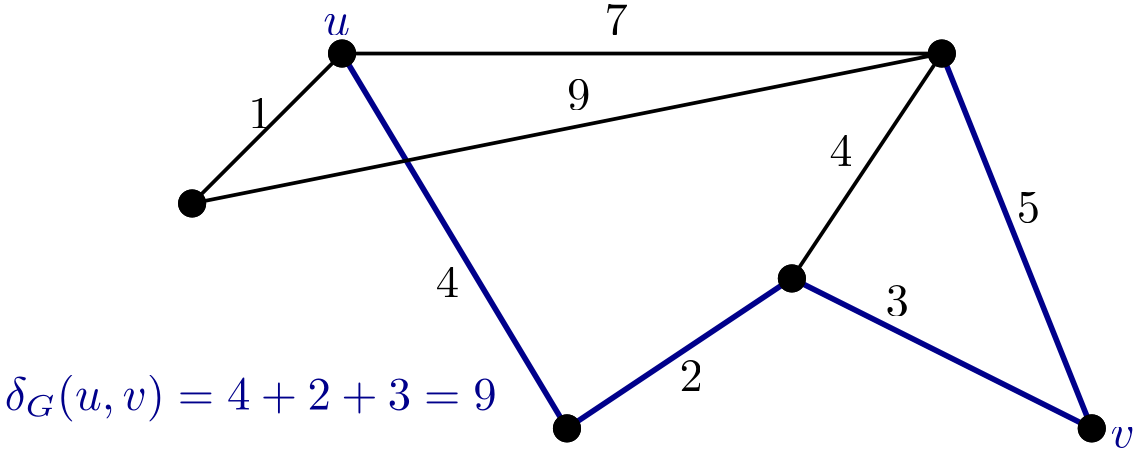
\includegraphics[width=0.75\textwidth]{images/wiener_index.png} % Replace with your own
	\end{center}
\end{frame}

\begin{frame}{Problem Statement: Geometric Spanning Trees}
	\textbf{Reference:} WADS 2023 ~\cite{article:geometric_spanning_trees_minimizing_wiener_index}

	\begin{enumerate}
		\item Input: A set $P$ of $n$ points in the plane.
		      \pause
		\item Goal: Construct a \textbf{spanning tree} on $P$ that minimizes the \textbf{Wiener index}.
		      \pause
		\item The weight function is defined as the Euclidean distance between points.
	\end{enumerate}
\end{frame}

\begin{frame}{Results Summary: Geometric Spanning Trees}
	\begin{itemize}
		\item Spanning tree of $P$ that minimizes the Wiener index is planar.
		      \pause
		\item When $P$ is in convex position, this can be solved in polynomial time.
		      \pause
		\item The hamiltonian path of $P$ that minimizes the Wiener index is not necessarily planar.
		      \pause
		\item Computing such a hamiltonian path is NP-Hard.
	\end{itemize}
\end{frame}

\begin{frame}{Minimum Spanning Tree (MST)}
	\begin{block}{Minimum Spanning Tree (MST)}
		A \textbf{minimum spanning tree} of a weighted undirected graph is a spanning tree that has the minimum total edge weight.
		\begin{itemize}
			\item The MST connects all vertices with the minimum total edge weight.
			\item It is unique if all edge weights are distinct.
		\end{itemize}
	\end{block}
\end{frame}

\begin{frame}{Euclidean Minimum Spanning Tree}
	\begin{block}{Euclidean Minimum Spanning Tree}
		The \textbf{Euclidean minimum spanning tree} (EMST) of a set of points in the Euclidean space is the minimum spanning tree where the edge weights are the Euclidean distances between points.
		\begin{itemize}
			\item The EMST can be computed in $O(n \log n)$ time.
			\item The EMST is unique if all points are distinct.
		\end{itemize}
	\end{block}
	\pause
	\vspace{0.5cm}

	Note: It can be shown that the EMST is a subgraph of special geometric graphs called \textbf{Delaunay triangulations} which are a dual of \textbf{Voronoi Diagrams} ~\cite{book:deberg_computational_geometry}.
\end{frame}

\begin{frame}{Euclidean Minimum Spanning Tree VS Wiener Index}
	\textbf{Question:} Is the EMST a good approximation for the spanning tree that minimizes the Wiener index?
	\vspace{0.3cm}
	\begin{itemize}
		\item \textbf{Answer:} No, see the code examples.
	\end{itemize}
	\vspace{0.5cm}

	\pause
	Aside: The EMST \textbf{could} be a good approximation or a heuristic for the spanning tree that minimizes the Wiener index. This may be worth exploring if we go the route of finding an approximation algorithm for the problem.
\end{frame}

\begin{frame}{Hypergraphs and their Wiener Index}
	\pause
	\begin{block}{Hypergraph}
		A \textbf{hypergraph} $H = (V, E)$ is a pair where $V$ is a set of vertices and $E$ is a set of hyperedges, each of which is a subset of $V$.
	\end{block}

	\pause
	\begin{block}{Distance in Hypergraphs}
		The \textbf{distance} between two vertices $u$ and $v$ in a hypergraph $H$ is defined as the minimum number of hyperedges in a chain connecting $u$ and $v$.
		\begin{itemize}
			\item A \textbf{chain} is a sequence of hyperedges where each consecutive pair shares at least one vertex.
			\item The distance is denoted as $\delta_H(u, v)$.
		\end{itemize}
	\end{block}

	\pause
	\begin{block}{k-uniform hypergraph}
		A hypergraph is \textbf{k-uniform} if every hyperedge has cardinality $k$.
	\end{block}
\end{frame}

\begin{frame}{Wiener Index in Hypergraphs}
	\pause
	\begin{block}{Wiener Index in Hypergraphs}
		The \textbf{Wiener index} of a hypergraph $H$ is defined as:
		\[
			W(H) = \sum_{u, v \in V} \delta_H(u, v)
		\]
	\end{block}
\end{frame}

\begin{frame}{Some facts about HyperGraphs}
	\begin{itemize}
		\pause
		\item Finding a spanning tree of general hypergraphs is NP-Complete, while spanning tree of 3-uniform hypergraphs has a polynomial time algorithm using matroid matching. ~\cite{article:spanning_tree_3_uniform_hypergraph}
		      \pause
		\item Finding a spanning tree of a $k$-uniform 2-regular hypergraph is NP-Complete for any $k \geq 4$. ~\cite{article:spanning_tree_k_uniform_2_regular_hypergraph}
	\end{itemize}
\end{frame}

\begin{frame}{Proposed Open Work: Wiener Index in Hypergraphs}
	\begin{itemize}
		\pause
		\item Focus: Define and study the \textbf{Wiener index} in various classes of hypergraphs.
		      \pause
		\item Distance: Find a suitable weighted/unweighted distance metric for hypergraphs.
		      \pause
		\item Goal: Characterize structures that minimize/maximize the Wiener index.
	\end{itemize}

	\pause
	Side note: We could also explore \textbf{spatially embedded hypergraphs}, drawing inspiration from ~\cite{article:geometric_spanning_trees_minimizing_wiener_index}, and their Wiener index.
\end{frame}

\begin{frame}[allowframebreaks]{References}
	\bibliography{references}
\end{frame}

\begin{frame}

	\begin{center}
		The end.

		\email
	\end{center}

	\begin{figure}[htb]
		\centering
	\end{figure}

\end{frame}

\end{document}
